\documentclass{article}

\usepackage{booktabs}
\usepackage{graphicx}
\usepackage{caption}
\usepackage{subcaption}

\graphicspath{{../dev/}}

\title{Strategy Analysis: Progressive Entry}
\author{Ivan Anich}

\begin{document}
\maketitle

Here I analyze a 'progressive entry' strategy in which a stock is sold short and then position size is added to each time it rises by 5\%. The adds double in size each time they occur. This trade strategy shows a lot of promise, but may require being able to afford many adds in order to achieve profits. At the end I analyze a variation of the strategy that may allow only 2 adds to be required, while still achieving meaningful profits.

\section{signal}

The signal analyzed is a rise of 20\% from the open, with a previous close between \$1 and \$2. 

\section{Strategy: Add Every 5\%, Exit at 11}

The default strategy assed is as follows: once the signal is observed (a rise of 20\% from open between 9:30 and 11) a short position is entered. Every time the stock rises another 5\%, a position twice as big as the last position is added to the overall position. So, if the initial position size is \$1,000, when a stock hits 20\% \$1000 worth of stock is short sold, at 25\% another \$2000, at 30\% another \$4,000 and so on. No limit to adds was introduced for this variation of the strategy (an analysis with a max of 2 adds is carried out below). Limits were not included at first in order to analyze the unrestricted potential of the strategy. Between February 26th and May 28th 2021, this strategy was executable across 65 trades.

\pagebreak

\subsection{Analysis:  Unlimited Adds, Exit at 11 a.m.}

\begin{table}
\caption{Performance of Default Strategy: Unlimited Adds, Exit at 11 a.m.}
\center{Overall}
\\[2ex]
\begin{tabular}{lcccc}
\hline
         &   0.1    &   0.9    &  median  & average   \\
\midrule
\midrule
constant & -0.0041  & 0.2483   & 0.0924   & 0.1020    \\
         & (0.0140) & (0.0271) & (0.0182) & (0.0123)  \\
N        & 65       & 65       & 65       & 65        \\
Win rate & 0.86     & 0.86     & 0.86     & 0.86      \\
\hline
\end{tabular}

\center{Winners}
\\[2ex]
\begin{tabular}{lcccc}
\hline
         &   0.25   &   0.75   &  median  & average   \\
\midrule
\midrule
constant & 0.0467   & 0.1611   & 0.1130   & 0.1220    \\
         & (0.0163) & (0.0199) & (0.0185) & (0.0123)  \\
N        & 56       & 56       & 56       & 56        \\
Win rate & 0.86     & 0.86     & 0.86     & 0.86      \\
\hline
\end{tabular}

\center{Losers}
\\[2ex]
\begin{tabular}{lcccc}
\hline
          &  0.25  &  0.75  &  median  & average   \\
\midrule
\midrule
constant  & 0.0041 & 0.0311 & 0.0280   & 0.0225    \\
          & (nan)  & (nan)  & (0.0140) & (0.0055)  \\
N         & 9      & 9      & 9        & 9         \\
Loss rate & 0.14   & 0.14   & 0.14     & 0.14      \\
\hline
\end{tabular}
\label{tab_strat}
\end{table}

The first thing to note about this strategy is that the doubling of position sizes every 5\%, or `progressive entry' as I call it, completely changes how we need to think about expected returns. The usual metric is not as informative as it was for other strategies we have analyzed. Table \ref{tab_strat} states that the average return on the trade is 10\%, but this does not take into account that some of those returns are on trades that were entered and only added to once or twice, and others are on trades that were added to 5, 6, or more times. The total position size on a trade with 5 adds is 64 times larger than the total size of a trade with an entry and no adds. The returns on the trades with many adds carry much more weight than those with fewer adds. Consequently, I calculated a weighted average of returns, where each return is weighted by its relative position size. 

\begin{figure}
	\center{Histogram of Trades by Number of Entries for Unlimited Adds, Exit at 11 a.m.}
	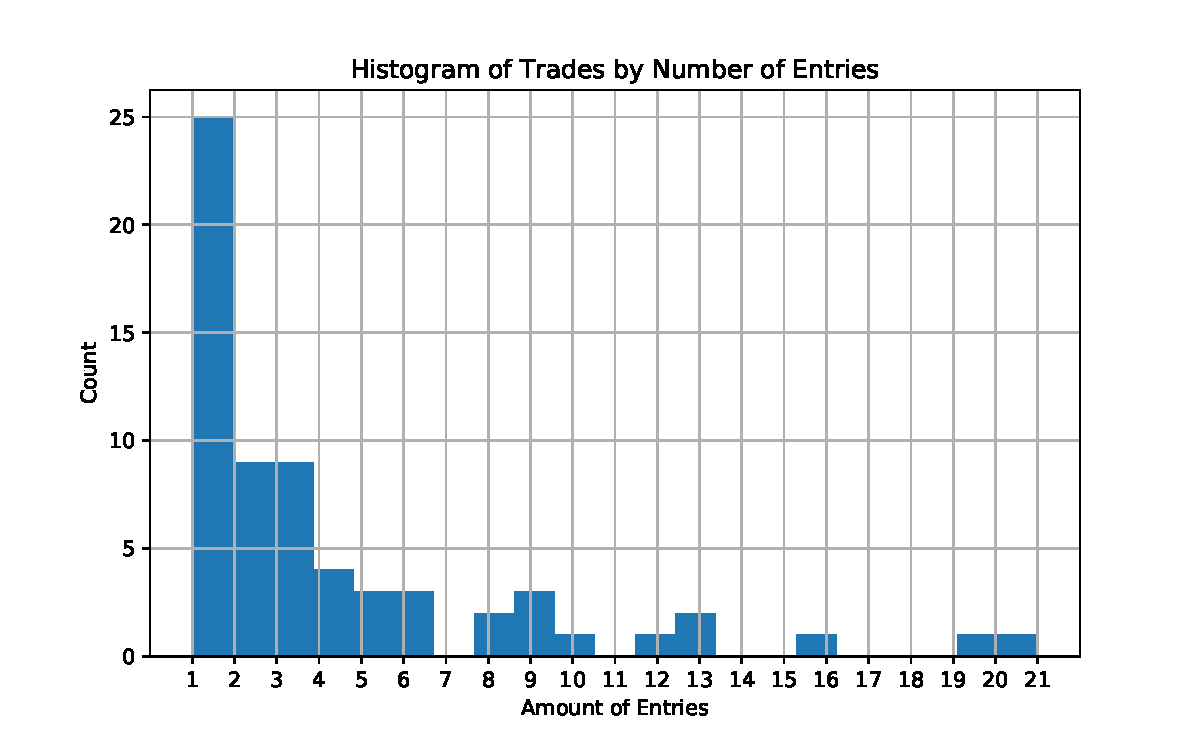
\includegraphics[width=\textwidth]{prog_entry_hist.pdf}
	\caption{This table shows counts of the numbers of trades that had a certain amount of entries. For example, it says that around 57 trades had only 1 entry, and that around 3 trades had 9 entries (fist entry and 8 adds).}
	\label{hist_strat}
	\end{figure}

The \textbf{weighted average return of this strategy is 29.7\%}. That is a stunning number, but it is a difficult one to achieve in practice. There is a high correlation between the number of adds and the return on a trade: the higher a stock rises above 20\%, the higher the return usually is. This is a strong support for the rationale behind this strategy. We are adding such that our costs are closely tracking the price, and every strong push up eventually has to come back down, even if only a little. But 47\% of trades have 2 or more adds (see figure \ref{hist_strat}. That means that 47\% have a position size at least 7 times larger than the initial entry. Numerous trades have even more adds. The weight of the return on a trade with 8 adds, of which there were 3, is 256 times larger than a trade with none. In order to be able to afford a progressive entry that eventually leads to positions sizes 256 times larger than the initial entry, the initial entry has to be very small, but this means that trades with few adds, of which there are many, will not have an affect on the portfolio. If you want to execute this strategy, we need to have very small initial position sizes so that you can afford 8 adds or more (256 times original entry size or more), but then you are acting in caution of a very rare event: only 10 trades had 8 adds or more (see figure \ref{hist_strat} again).

But this is something that you foresaw when you thought of limiting the number of adds to two. In the spirit of such thought, I provide figure \ref{w_avg_strat}, which displays the weighted average return for various add limits. As you can see, as we increase the limit to the number of adds we can put into a trade, the weighted return increases. Unfortunately, the weighted average return for a limit of 2 adds is insignificantly different from zero. 

Figure \ref{3plot_strat} provides further breakdown of the strategy. The top panel, unweighted expected return for each add limit, provides an excellent illustration of the difference between weighted and unweighted return. As the number of adds we are allowed to make increases, the unweighted return doesn't change very much, but the weighted return as shown in figure \ref{w_avg_strat} becomes far larger than the unweighted return.

	\begin{figure}
	\center{Weighted Average Returns for Unlimited Adds, Exit at 11 a.m.}
	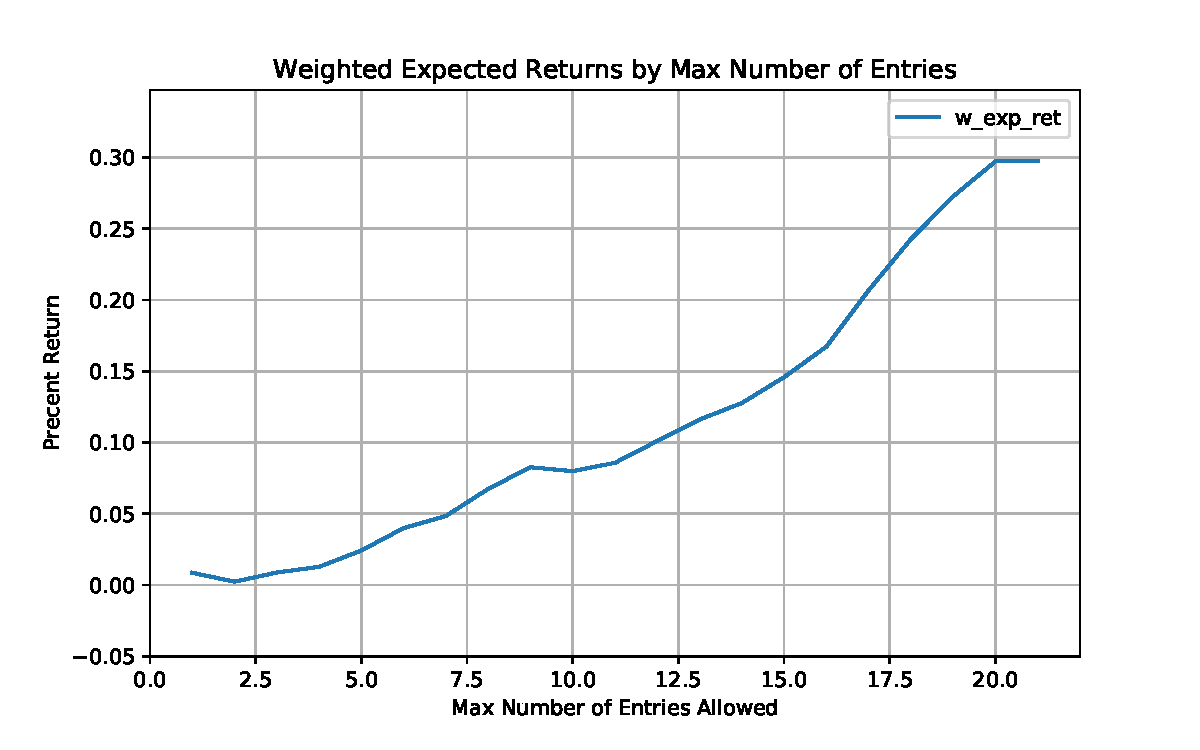
\includegraphics[width=\textwidth]{prog_entry_w_avg.pdf}
	\caption{This plot shows the weighted expected return to a limited version of the main strategy. Returns are weighted by their position size. Trades with more adds have higher weight. The returns on trades with higher weight have a larger affect on the weighted average than they would in an unweighted average. The x-axis displays the maximum number of entries allowed in a single trade. In the unlimited case, a trade can be entered each time it rises 5\%. But in the case where adds are limited to 4, the total number of entries allowed in any stock is 5 (first entry then 4 adds). So this plot says that when the maximum amount of entries is 5 (i.e. at most 4 adds) the weighted returns were around 2.5\%. When the amount of entries is limited to 5 (first entry, 4 adds), stocks that rise more than 25\% beyond the signal of 20\% are not added to beyond the first 4 adds.}
	\label{w_avg_strat}
	\end{figure}
	
	\begin{figure}
	\center{Win Rate, Unweighted Average Return, and Average Win/Loss for Unlimited Adds, Exit at 11 a.m.}
	
	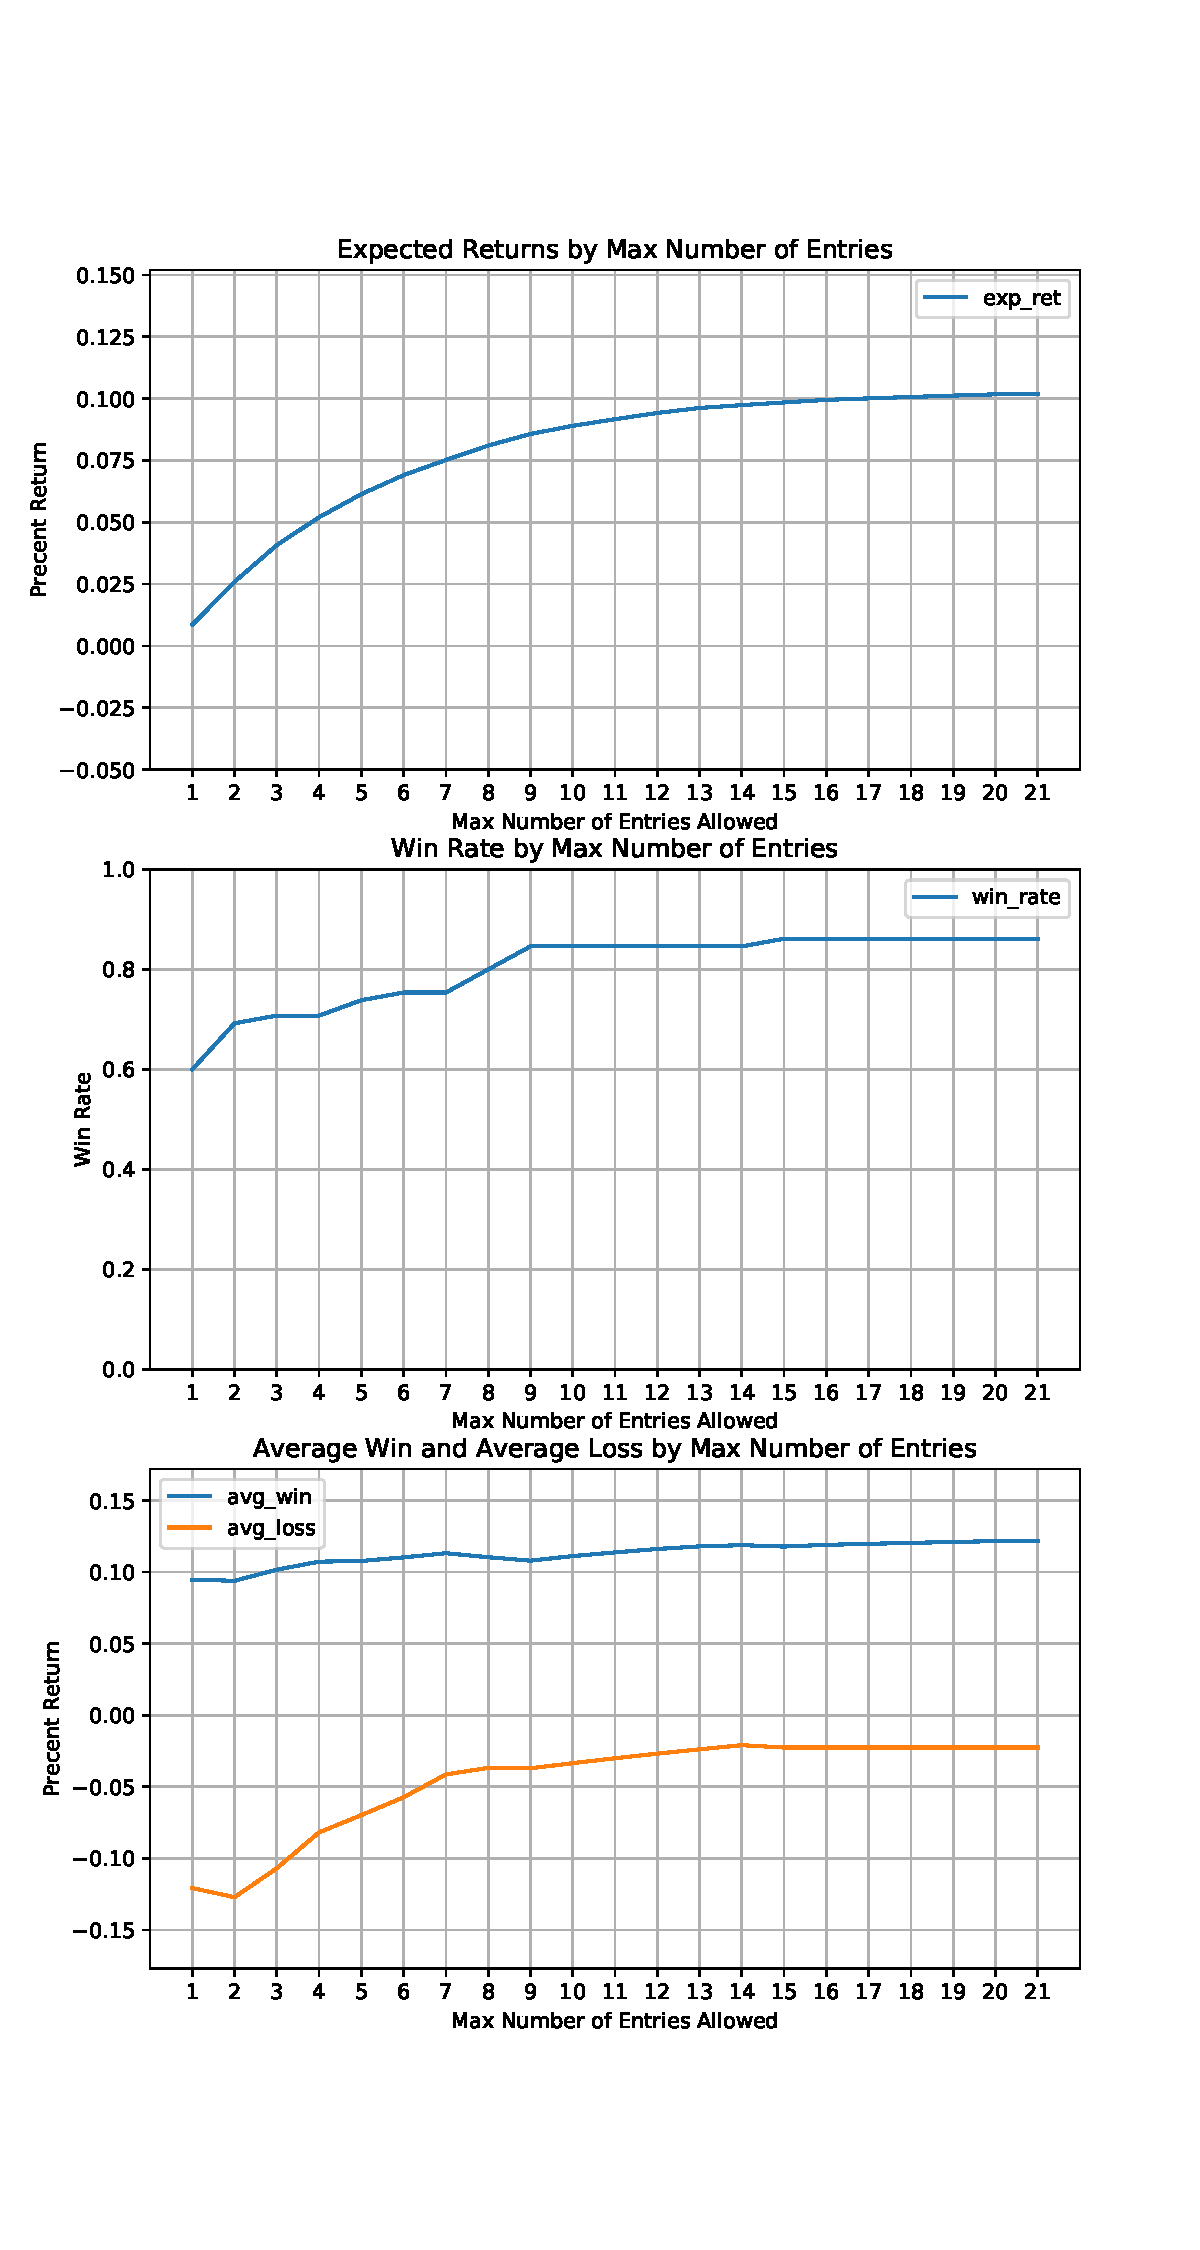
\includegraphics[width=0.6\textwidth]{prog_entry_3plot.pdf}
	\caption{The x-axis displays the maximum number of entries allowed in a single trade. In the unlimited case, a trade can be entered each time it rises 5\%. But in the case where adds are limited to 4, the total number of entries allowed in any stock is 5 (first entry then 4 adds). So the top panel says that when the maximum amount of entries is 5 (i.e. at most 4 adds) the returns were around 5.75\%. When the amount of entries is limited to 5 (first entry, 4 adds), stocks that rise more than 25\% beyond the signal of 20\% are not added to beyond the first 4 adds.}
	\label{3plot_strat}
	\end{figure}
	
	
\pagebreak

\section{Alternate Strategy A: Adds Limited to 2, Exit at 11}

To analyze a more feasible strategy, I looked more in depth at a limit of 2 adds, with an exit still at 11 a.m. 47\% of trades hit this limit. 

\subsection{Analysis}

	
\begin{table}
\caption{Performance of Max 3 Adds, Exit at 11 a.m.}
\center{Overall}
\\[2ex]
\begin{tabular}{lcccc}
\hline
         &   0.1    &   0.9    &  median  & average   \\
\midrule
\midrule
constant & -0.1434  & 0.1709   & 0.0468   & 0.0408    \\
         & (0.0444) & (0.0204) & (0.0191) & (0.0160)  \\
N        & 65       & 65       & 65       & 65        \\
Win rate & 0.71     & 0.71     & 0.71     & 0.71      \\
\hline
\end{tabular}

\center{Winners}
\\[2ex]
\begin{tabular}{lcccc}
\hline
         &   0.25   &   0.75   &  median  & average   \\
\midrule
\midrule
constant & 0.0353   & 0.1593   & 0.0919   & 0.1018    \\
         & (0.0163) & (0.0220) & (0.0167) & (0.0116)  \\
N        & 46       & 46       & 46       & 46        \\
Win rate & 0.71     & 0.71     & 0.71     & 0.71      \\
\hline
\end{tabular}

\center{Losers}
\\[2ex]
\begin{tabular}{lcccc}
\hline
          &  0.25  &  0.75  &  median  & average   \\
\midrule
\midrule
constant  & 0.0307 & 0.1774 & 0.0657   & 0.1069    \\
          & (nan)  & (nan)  & (0.0391) & (0.0242)  \\
N         & 19     & 19     & 19       & 19        \\
Loss rate & 0.29   & 0.29   & 0.29     & 0.29      \\
\hline
\end{tabular}
\label{tab_strat_lim3}
\end{table}

While more feasible, this strategy is not profitable. I want to note that a constant exit time may be an inefficient tactic. It may be better to bracket a trade with stop losses so that adds are automatically added at the appropriate 5\% intervals, and a profit threshold is guaranteed as well. 

The unweighted expected return is 4\%, the \textbf{weighted expected return is only 0.9\%}. Figure \ref{hist_by_entry_strat_lim3} breaks down how many returns of certain magnitudes occurred for trades with no adds, 1 add, and 2 adds. It shows that among trades that hit the add limit, 17 had returns between 0\% and 20\%, while 14 had returns between -50\% and 0\%. Given that these limited trades have a position size 7 times larger than the initial entry size, these losses have a big effect on the profitability of this strategy.

	\begin{figure}
	\center{Histogram of Percent Return by Number of Entries for Max 2 Adds, Exit at 11 a.m.}
	
	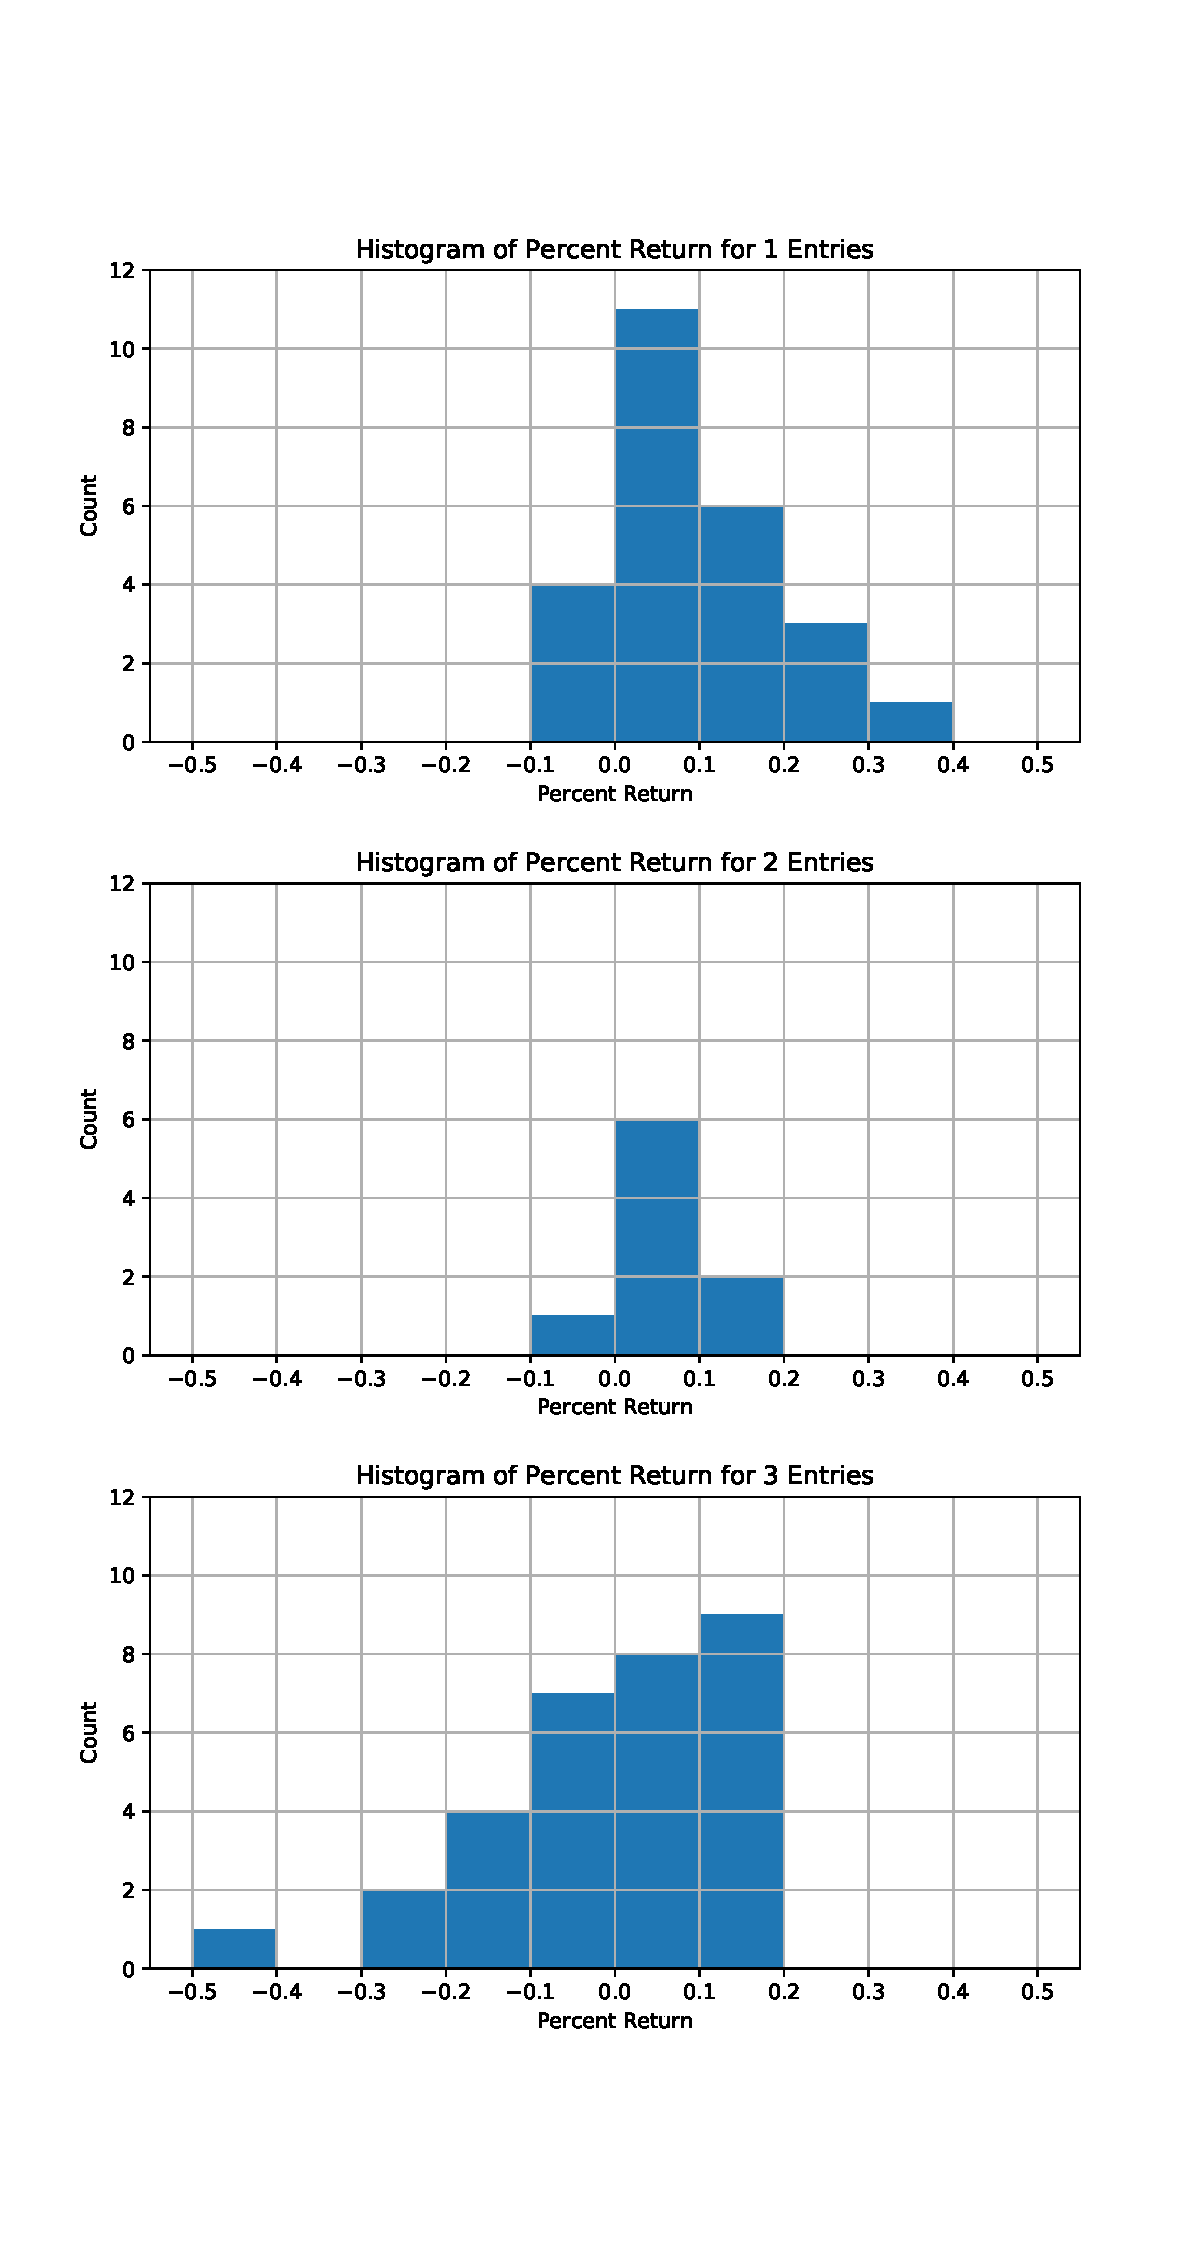
\includegraphics[width=0.6\textwidth]{prog_entry_lim3_hist_by_entry.pdf}
	\caption{This table shows counts of the numbers of trades that had certain percent returns. For example, the top panel says that 11 trades with only 1 entry (the first entry) had a return between 0\% and 10\%.}
	\label{hist_by_entry_strat_lim3}
	\end{figure}
	

\pagebreak

\section{Alternate Strategy B: Adds limited to 2, Exit at Close}

As a bit of exploratory work, I looked at how things would change if we exited at close, while still limited to two adds. I was motivated to do this when I looked at figure \ref{w_avg_strat_exit4}, which displays the weighted expected returns for each add limit for an exit at close. Over all, it seems it is far more profitable to add throughout the day and exit at close, including for a limit of only 2 adds. 

This strategy was available in 146 trades between February 26th and May 28th of 2021. 41\% of trades hit the 2 add limit (see figure \ref{hist_strat_exit4}). 

\begin{figure}
	\center{Weighted Average Returns for Unlimited Adds, Exit at Close}
	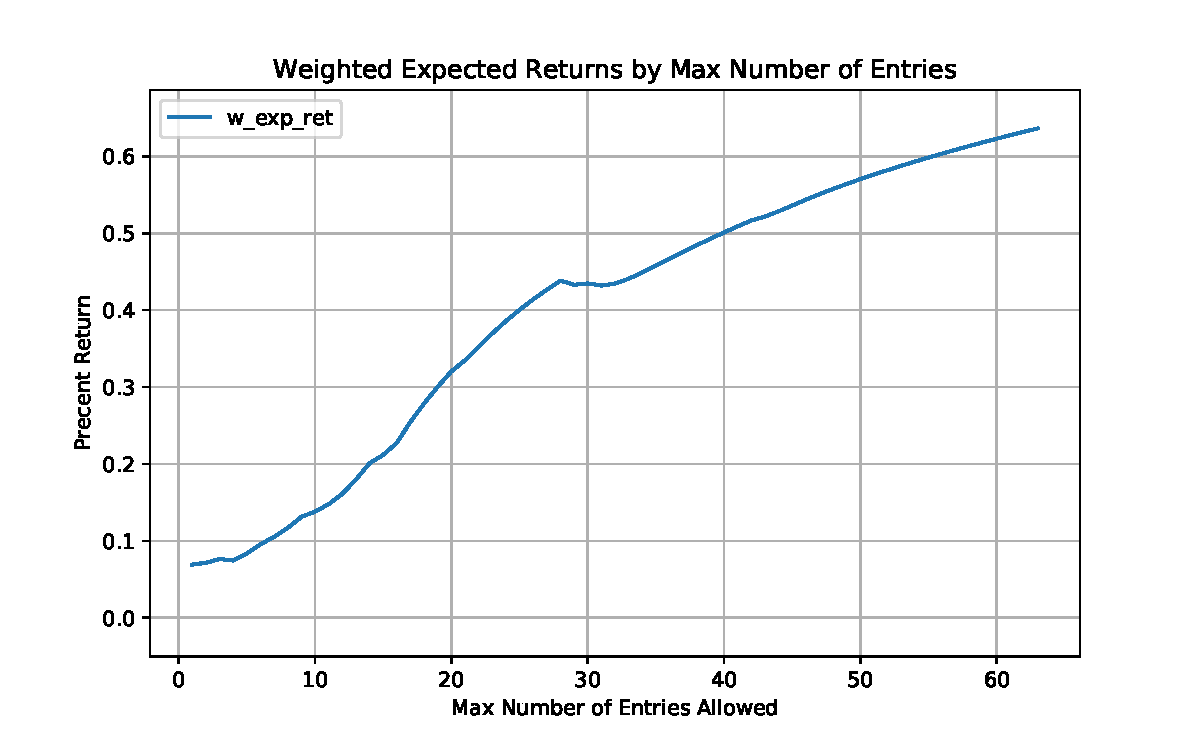
\includegraphics[width=\textwidth]{prog_entry_exit4_w_avg.pdf}
	\caption{This plot shows the weighted expected return to a limited version of the main strategy. Returns are weighted by their position size. Trades with more adds have higher weight. The returns on trades with higher weight have a larger affect on the weighted average than they would in an unweighted average. The x-axis displays the maximum number of entries allowed in a single trade. In the unlimited case, a trade can be entered each time it rises 5\%. But in the case where adds are limited to 4, the total number of entries allowed in any stock is 5 (first entry then 4 adds). So this plot says that when the maximum amount of entries is 5 (i.e. at most 4 adds) the weighted returns were around 8\%. When the amount of entries is limited to 5 (first entry, 4 adds), stocks that rise more than 25\% beyond the signal of 20\% are not added to beyond the first 4 adds.}
	\label{w_avg_strat_exit4}
	\end{figure}

	\begin{figure}
	\center{Histogram of Trades by Number of Entries for Unlimited Adds, Exit at Close}
	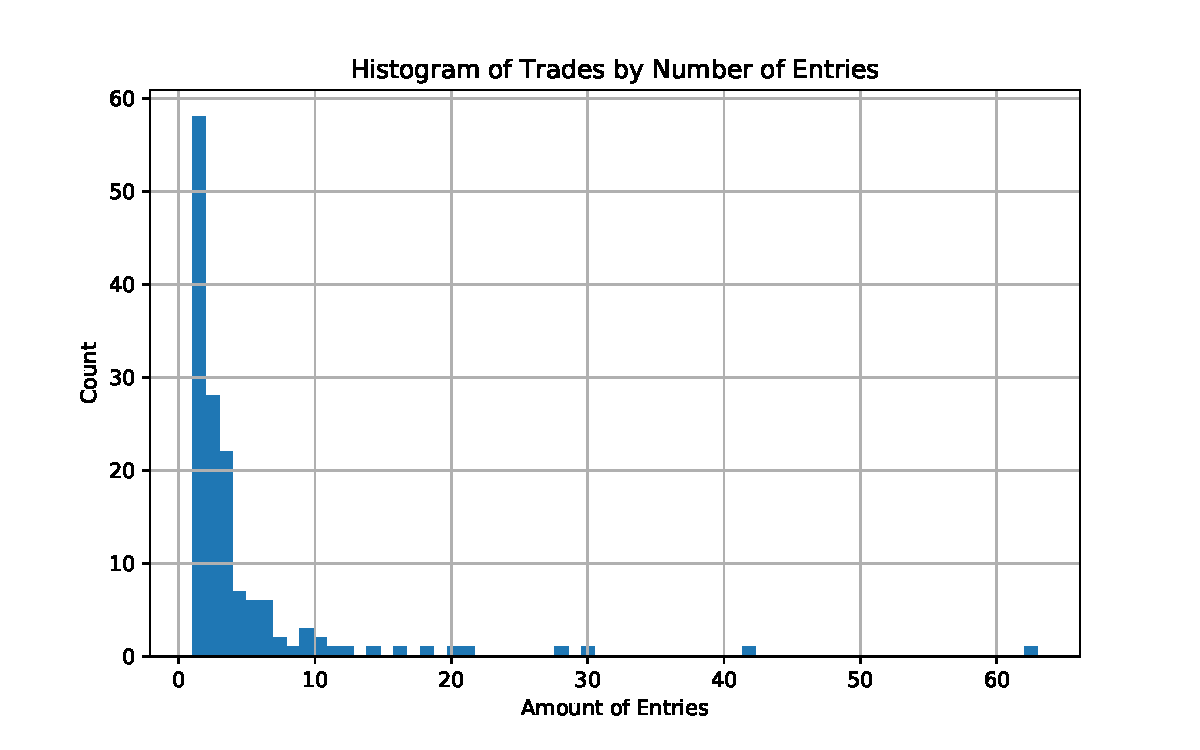
\includegraphics[width=\textwidth]{prog_entry_exit4_hist.pdf}
	\caption{This table shows counts of the numbers of trades that had a certain amount of entries. For example, it says that around 57 trades had only 1 entry, and that around 3 trades had 9 entries (fist entry and 8 adds).}
	\label{hist_strat_exit4}
	\end{figure}

\subsection{Analysis}

	\begin{table}
\caption{Performance of Max 2 Adds, Exit at Close}
\center{Overall}
\\[2ex]
\begin{tabular}{lcccc}
\hline
         &   0.1    &   0.9    &  median  & average   \\
\midrule
\midrule
constant & -0.0307  & 0.1917   & 0.1110   & 0.0969    \\
         & (0.0331) & (0.0076) & (0.0083) & (0.0085)  \\
N        & 146      & 146      & 146      & 146       \\
Win rate & 0.89     & 0.89     & 0.89     & 0.89      \\
\hline
\end{tabular}

\center{Winners}
\\[2ex]
\begin{tabular}{lcccc}
\hline
         &   0.25   &   0.75   &  median  & average   \\
\midrule
\midrule
constant & 0.0844   & 0.1610   & 0.1211   & 0.1241    \\
         & (0.0073) & (0.0070) & (0.0074) & (0.0053)  \\
N        & 130      & 130      & 130      & 130       \\
Win rate & 0.89     & 0.89     & 0.89     & 0.89      \\
\hline
\end{tabular}

\center{Losers}
\\[2ex]
\begin{tabular}{lcccc}
\hline
          &  0.25  &  0.75  &  median  & average   \\
\midrule
\midrule
constant  & 0.0516 & 0.1774 & 0.0916   & 0.1247    \\
          & (nan)  & (nan)  & (0.0455) & (0.0264)  \\
N         & 16     & 16     & 16       & 16        \\
Loss rate & 0.11   & 0.11   & 0.11     & 0.11      \\
\hline
\end{tabular}
\label{tab_strat_lim3_exit4}
\end{table}

The unweighted average return is 9.7\%, \textbf{the weighted average return is 7.6'\%}. The win rate is also very high at 89\%. An exciting feature of this strategy is that a far higher number of the trades with the greatest weight are winners (see third panel in figure \ref{hist_by_entry_strat_exit4}), and the big losses for these trades occur far less often. This means that we can play a relatively larger initial sizes, and so earn meaningful profits for smaller trades while still being able to afford the maximum position size.   

	
	\begin{figure}
	\center{Histogram of Percent Return by Number of Entries for Max 2 Adds, Exit at Close}
	
	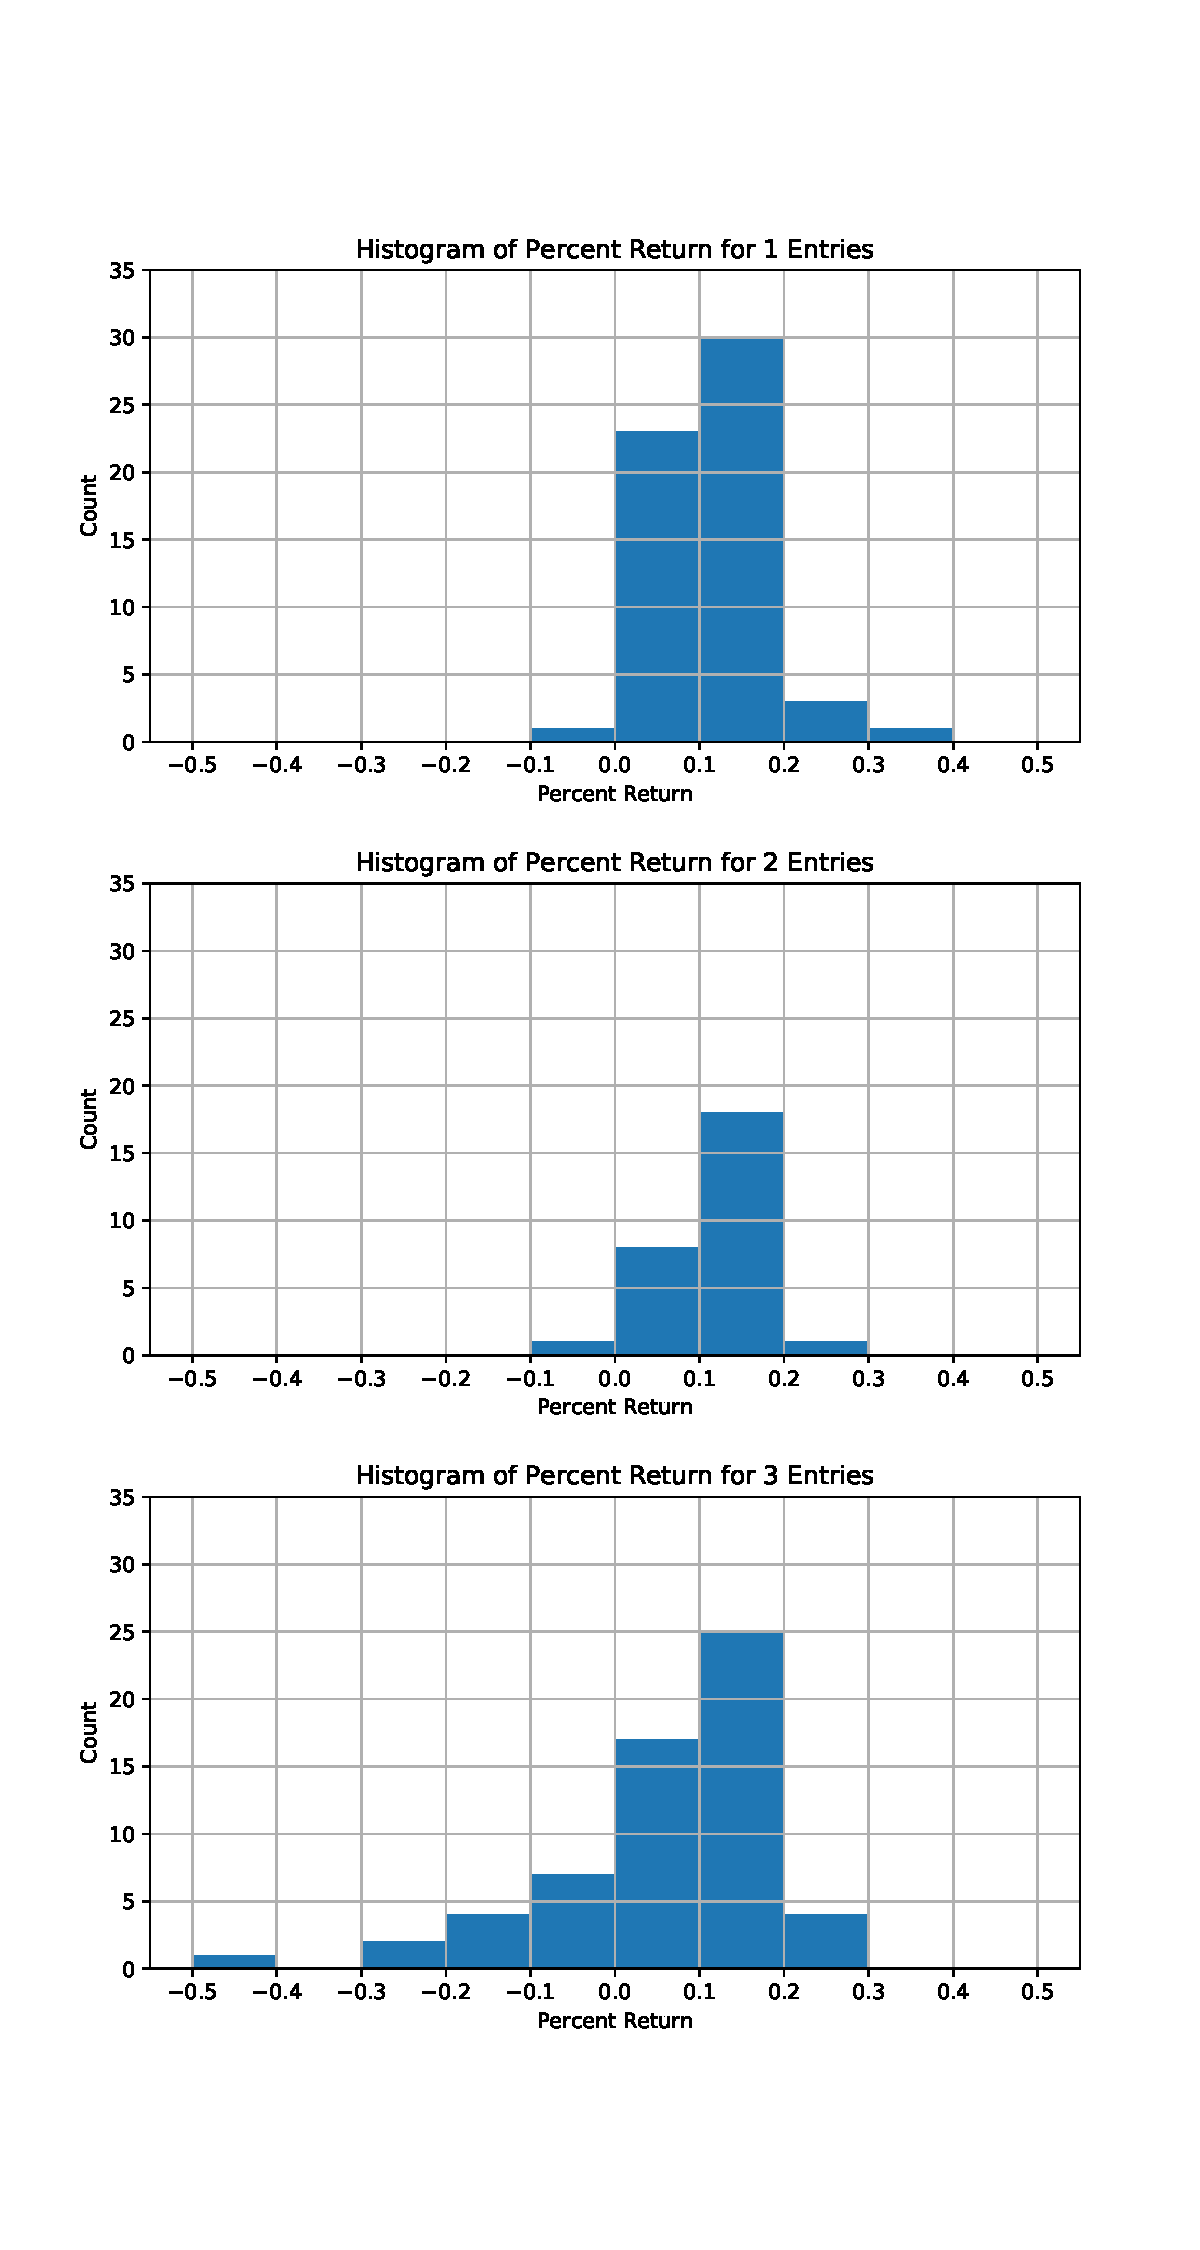
\includegraphics[width=0.6\textwidth]{prog_entry_lim3_exit4_hist_by_entry.pdf}
	\caption{This table shows counts of the numbers of trades that had certain percent returns. For example, the top panel says that 23 trades with only 1 entry (the first entry) had a return between 0\% and 10\%.}
	\label{hist_by_entry_strat_exit4}
	\end{figure}
	
\end{document}